
%%% main document {{{

\documentclass[
a4paper,     %% defines the paper size: a4paper (default), a5paper, letterpaper, ...
% landscape,   %% sets the orientation to landscape
% twoside,     %% changes to a two-page-layout (alternatively: oneside)
% twocolumn,   %% changes to a two-column-layout
% headsepline, %% add a horizontal line below the column title
% footsepline, %% add a horizontal line above the page footer
% titlepage,   %% only the titlepage (using titlepage-environment) appears on the first page (alternatively: notitlepage)
% parskip,     %% insert an empty line between two paragraphs (alternatively: halfparskip, ...)
% leqno,       %% equation numbers left (instead of right)
% fleqn,       %% equation left-justified (instead of centered)
% tablecaptionabove, %% captions of tables are above the tables (alternatively: tablecaptionbelow)
% draft,       %% produce only a draft version (mark lines that need manual edition and don't show graphics)
% 10pt         %% set default font size to 10 point
% 11pt         %% set default font size to 11 point
12pt         %% set default font size to 12 point
]{scrartcl}  %% article, see KOMA documentation (scrguide.dvi)



%%%%%%%%%%%%%%%%%%%%%%%%%%%%%%%%%%%%%%%%%%%%%%%%%%%%%%%%%%%%%%%%%%%%%%%%%%%%%%%%
%%%
%%% packages
%%%

%%%
%%% encoding and language set
%%%

%%% ngerman: language set to new-german
\usepackage{ngerman}

%%% babel: language set (can cause some conflicts with package ngerman)
%%%        use it only for multi-language documents or non-german ones
%\usepackage[ngerman]{babel}

%%% inputenc: coding of german special characters
\usepackage[utf8]{inputenc}

%%% fontenc, ae, aecompl: coding of characters in PDF documents
\usepackage[T1]{fontenc}
\usepackage{ae,aecompl}

%%%
%%% technical packages
%%%

%%% amsmath, amssymb, amstext: support for mathematics
%\usepackage{amsmath,amssymb,amstext}

%%% psfrag: replace PostScript fonts
\usepackage{psfrag}

%%% listings: include programming code
%\usepackage{listings}

%%% units: technical units
\usepackage{units}

%%% tiefgestellte zahlen
\usepackage{subscript}

%%% mathefoo
\usepackage{amsmath}


\usepackage{xcolor}
% TikZ-Bibliotheken
\usepackage{tikz}
 \usetikzlibrary{backgrounds}
 \usetikzlibrary{matrix}
 \usetikzlibrary{circuits.ee.IEC}
 \usetikzlibrary{positioning}
 
 
%Hintergrundstyle - optional
\tikzstyle{background rectangle}=
  [thick,draw=\lightgray, fill=white!99!black, rounded corners]
 
%Volt- und Amperemeter festlegen:
\tikzset{circuit declare symbol = ammeter}
\tikzset{set ammeter graphic ={draw,generic circle IEC, minimum size=5mm,info=center:A}}
\tikzset{circuit declare symbol = voltmeter}
\tikzset{set voltmeter graphic ={draw,generic circle IEC, minimum size=5mm,info=center:V}}
\tikzset{circuit declare symbol = generator}
\tikzset{set generator graphic ={draw,rectangle ee, minimum size=5mm,info=center:G}}
% Spannungs und Strompfeile
\tikzset{
  Pfeil/.style={thick,shorten >=#1,shorten <=#1,->}, % für Peile
  UPfeil/.style={blue,Pfeil=#1,font={\sffamily\itshape}},% für Spannungspfeile
  IPfeil/.style={red,Pfeil=#1,font={\ttfamily\itshape}} % für Strompfeile
}


%%%
%%% layout
%%%

%%% scrpage2: KOMA heading and footer
%%% Note: if you don't use this package, please remove 
%%%       \pagestyle{scrheadings} and corresponding settings
%%%       below too.
\usepackage[automark]{scrpage2}


%%%
%%% PDF
%%%

\usepackage{ifpdf}

%%% Should be LAST usepackage-call!
%%% For docu on that, see reference on package ``hyperref''
\ifpdf%   (definitions for using pdflatex instead of latex)

  %%% graphicx: support for graphics
  %\usepackage[pdftex]{graphicx}

  \pdfcompresslevel=9

  %%% hyperref (hyperlinks in PDF): for more options or more detailed
  %%%          explanations, see the documentation of the hyperref-package
  \usepackage[%
    %%% general options
    pdftex=true,      %% sets up hyperref for use with the pdftex program
    %plainpages=false, %% set it to false, if pdflatex complains: ``destination with same identifier already exists''
    %
    %%% extension options
    backref,      %% adds a backlink text to the end of each item in the bibliography
    pagebackref=false, %% if true, creates backward references as a list of page numbers in the bibliography
    colorlinks=true,   %% turn on colored links (true is better for on-screen reading, false is better for printout versions)
    %
    %%% PDF-specific display options
    bookmarks=true,          %% if true, generate PDF bookmarks (requires two passes of pdflatex)
    bookmarksopen=false,     %% if true, show all PDF bookmarks expanded
    bookmarksnumbered=false, %% if true, add the section numbers to the bookmarks
    %pdfstartpage={1},        %% determines, on which page the PDF file is opened
    pdfpagemode=None         %% None, UseOutlines (=show bookmarks), UseThumbs (show thumbnails), FullScreen
  ]{hyperref}


  %%% provide all graphics (also) in this format, so you don't have
  %%% to add the file extensions to the \includegraphics-command
  %%% and/or you don't have to distinguish between generating
  %%% dvi/ps (through latex) and pdf (through pdflatex)
  \DeclareGraphicsExtensions{.pdf}

\else %else   (definitions for using latex instead of pdflatex)

  \usepackage[dvips]{graphicx}

  \DeclareGraphicsExtensions{.eps}

  \usepackage[%
    dvips,           %% sets up hyperref for use with the dvips driver
    colorlinks=false %% better for printout version; almost every hyperref-extension is eliminated by using dvips
  ]{hyperref}

\fi


%%% sets the PDF-Information options
%%% (see fields in Acrobat Reader: ``File -> Document properties -> Summary'')
%%% Note: this method is better than as options of the hyperref-package (options are expanded correctly)
\hypersetup{
  pdftitle={}, %%
  pdfauthor={}, %%
  pdfsubject={}, %%
  pdfcreator={Accomplished with LaTeX2e and pdfLaTeX with hyperref-package.}, %% 
  pdfproducer={}, %%
  pdfkeywords={} %%
}


%%%%%%%%%%%%%%%%%%%%%%%%%%%%%%%%%%%%%%%%%%%%%%%%%%%%%%%%%%%%%%%%%%%%%%%%%%%%%%%%
%%%
%%% user defined commands
%%%

%%% \mygraphics{}{}{}
%% usage:   \mygraphics{width}{filename_without_extension}{caption}
%% example: \mygraphics{0.7\textwidth}{rolling_grandma}{This is my grandmother on inlinescates}
%% requires: package graphicx
%% provides: including centered pictures/graphics with a boldfaced caption below
%% 
\newcommand{\mygraphics}[3]{
  \begin{center}
    \includegraphics[width=#1, keepaspectratio=true]{#2} \\
    \textbf{#3}
  \end{center}
}

%%%%%%%%%%%%%%%%%%%%%%%%%%%%%%%%%%%%%%%%%%%%%%%%%%%%%%%%%%%%%%%%%%%%%%%%%%%%%%%%
%%%
%%% define the titlepage
%%%

% \subject{}   %% subject which appears above titlehead
% \titlehead{} %% special heading for the titlepage

%%% title
\title{Messbericht Reihenschaltung}

%%% author(s)
\author{Felix Schiller \\ Sebastian Littau \\ E1FS2}

%%% date
\date{Reutlingen, am \today{}}

% \publishers{}

% \thanks{} %% use it instead of footnotes (only on titlepage)

% \dedication{} %% generates a dedication-page after titlepage


%%% uncomment following lines, if you want to:
%%% reuse the maketitle-entries for hyperref-setup
%\newcommand\org@maketitle{}
%\let\org@maketitle\maketitle
%\def\maketitle{%
%  \hypersetup{
%    pdftitle={\@title},
%    pdfauthor={\@author}
%    pdfsubject={\@subject}
%  }%
%  \org@maketitle
%}


%%%%%%%%%%%%%%%%%%%%%%%%%%%%%%%%%%%%%%%%%%%%%%%%%%%%%%%%%%%%%%%%%%%%%%%%%%%%%%%%
%%%
%%% set heading and footer
%%%

%%% scrheadings default: 
%%%      footer - middle: page number
\pagestyle{scrheadings}

%%% user specific
%%% usage:
%%% \position[heading/footer for the titlepage]{heading/footer for the rest of the document}

%%% heading - left
\ihead[]{Schiller, Felix \\ Littau, Sebastian}

%%% heading - center
\chead[]{Messbericht \\Reihenschaltung}

%%% heading - right
\ohead[]{\thepage}

%%% footer - left
% \ifoot[]{}

%%% footer - center
% \cfoot[]{}

%%% footer - right
% \ofoot[]{}



%%%%%%%%%%%%%%%%%%%%%%%%%%%%%%%%%%%%%%%%%%%%%%%%%%%%%%%%%%%%%%%%%%%%%%%%%%%%%%%%
%%%
%%% begin document
%%%

\begin{document}

% \pagenumbering{roman} %% small roman page numbers

%%% include the title
% \thispagestyle{empty}  %% no header/footer (only) on this page
\maketitle

%%% start a new page and display the table of contents
\newpage
\tableofcontents

%%% start a new page and display the list of figures
% \newpage
% \listoffigures

%%% start a new page and display the list of tables
% \newpage
% \listoftables

%%% display the main document on a new page 
% \newpage

% \pagenumbering{arabic} %% normal page numbers (include it, if roman was used above)

%%%%%%%%%%%%%%%%%%%%%%%%%%%%%%%%%%%%%%%%%%%%%%%%%%%%%%%%%%%%%%%%%%%%%%%%%%%%%%%%
%%%
%%% begin main document
%%% structure: \section \subsection \subsubsection \paragraph \subparagraph
%%%
\section{Messaufgabe}
An einer Reihenschaltung von 4 Widerständen soll durch Messung ermittelt werden, wie sich 
\begin{enumerate}
\begin{enumerate}
	\item die Ströme zwischen den einzelnen Bauteilen und 
	\item die Spannungen an den einzelnen Bauteilen verhalten. 
\end{enumerate}
\end{enumerate}
Die messtechnisch gewonnenen Ergebnisse sind so zu verallgemeinern, dass sie auf beliebige Widerstandsreihenschaltungen anwendbar sind. \\
Mit den gewonnenen Erkenntnissen ist die zu Beginn gestellte Problemstellung zu bearbeiten.

\section{Stromabhängigkeit}
\subsection{Messschaltung zur Bestimmung der Ströme zwischen den Bauteilen}

\begin{center}
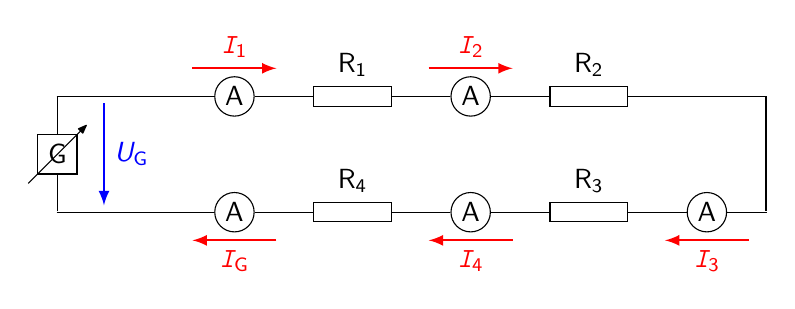
\begin{tikzpicture}[%show background rectangle,
circuit ee IEC, circuit symbol lines/.style={draw,thick},
font=\sffamily\upshape,
>=latex % Voreinstellung für Pfeilspitzen
]
\matrix (S) [
  matrix of nodes, nodes in empty cells,
  inner sep=0pt, outer sep=-.5\pgflinewidth,
  column sep=15mm, row sep = 7mm,
  nodes={minimum width=0pt}
  ]
{
  &&&&&&  \\
  &&&&&&  \\
  &&&&&&  \\
};
 
 
%Orientierungshilfen
%\foreach \j in {1,...,3}
% \foreach \k in {1,...,7}{%
%\node[text=lightgray] at (S-\j-\k){+}; % Orientierungshilfe +
%\node[red, left] at (S-\j-1){\j}; %Orientierungshilfe Zeilennummer
%\node[red, above] at (S-1-\k){\k}; %Orientierungshilfe Spaltennummer  
%};%
 

%Bauteile
\draw (S-3-1) to  [generator=adjustable'](S-1-1);
\draw (S-1-3) to  [resistor={info=R$_\mathsf{1}$, name=Wstd}](S-1-4);
\draw (S-1-2) to  [ammeter ={name=AM1}](S-1-3);
\draw (S-1-5) to  [resistor={info=R$_\mathsf{2}$, name=Wstd}](S-1-6);
\draw (S-1-4) to  [ammeter ={name=AM2}](S-1-5);
\draw (S-3-5) to  [resistor={info=R$_\mathsf{3}$, name=Wstd}](S-3-6);
\draw (S-3-6) to  [ammeter ={name=AM3}](S-3-7);
\draw (S-3-3) to  [resistor={info=R$_\mathsf{4}$, name=Wstd}](S-3-4);
\draw (S-3-4) to  [ammeter ={name=AM4}](S-3-5);
\draw (S-3-2) to  [ammeter ={name=AMg}](S-3-3);

%Spannungspfeile
%Spannungspfeil der Quelle / des Voltmeters
\draw[UPfeil=0.25em] ([xshift=6mm]S-1-1.east) -- ([xshift=6mm]S-3-1.east) node[midway, right]{U$\mathsf{_{G}}$};

%Strompfeile
\draw[IPfeil=-1em]([yshift=.5em]AM1.north west) -- node [above]{I$\mathsf{_1}$}([yshift=.5em]AM1.north east);
\draw[IPfeil=-1em]([yshift=.5em]AM2.north west) -- node [above]{I$\mathsf{_2}$}([yshift=.5em]AM2.north east); 
\draw[IPfeil=-1em]([yshift=-.5em]AM3.south east) -- node [below]{I$\mathsf{_3}$}([yshift=-.5em]AM3.south west); 
\draw[IPfeil=-1em]([yshift=-.5em]AM4.south east) -- node [below]{I$\mathsf{_4}$}([yshift=-.5em]AM4.south west);
\draw[IPfeil=-1em]([yshift=-.5em]AMg.south east) -- node [below]{I$\mathsf{_G}$}([yshift=-.5em]AMg.south west);
 
%Leiterbahnen
\draw (S-1-1) -- (S-1-2);
\draw (S-1-6) -- (S-1-7);
\draw (S-1-7) -- (S-3-7);
\draw (S-3-1) -- (S-3-2);
 
 
 
\end{tikzpicture}
\end{center}

\subsection{Aufbau der Schaltung}

\textbf{Textbeschreibung der Schaltung}

\subsection{Messwerte und Zusammenhänge}

In der oben beschrieben Schaltung wurden die folgenden Ströme gemessen.
\begin{center}
  \begin{tabular}{ l | c | c | c | c | c}
    \hline
    Strom      & I\textsubscript{1} & I\textsubscript{2} & I\textsubscript{3} & I\textsubscript{4} & I\textsubscript{G} \\ \hline
    Wert in mA & 6 & 6 & 6 & 6 & 6 \\
    \hline
  \end{tabular}
\end{center}
Der Strom ist in allen Widerständen gleich groß. Oder Allgemeiner ausgedrückt: In einer Reihenschaltung ist der Strom an jeder Stelle gemessen gleich groß.

\section{Spannungsabhängigkeit}
\subsection{Messschaltung zur Messung der Spannung über die einzelnen Bauteile}

\begin{center}
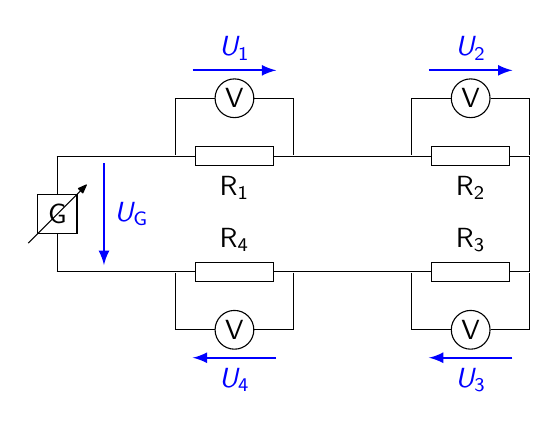
\begin{tikzpicture}[%show background rectangle,
circuit ee IEC, circuit symbol lines/.style={draw,thick},
font=\sffamily\upshape,
>=latex % Voreinstellung für Pfeilspitzen
]
\matrix (S) [
  matrix of nodes, nodes in empty cells,
  inner sep=0pt, outer sep=-.5\pgflinewidth,
  column sep=15mm, row sep = 7mm,
  nodes={minimum width=0pt}
  ]
{
  &&&&  \\
  &&&&  \\
  &&&&  \\
  &&&&  \\
  &&&&  \\
};
 
 
%Orientierungshilfen
%\foreach \j in {1,...,5}
% \foreach \k in {1,...,5}{%
%\node[text=lightgray] at (S-\j-\k){+}; % Orientierungshilfe +
%\node[red, left] at (S-\j-1){\j}; %Orientierungshilfe Zeilennummer
%\node[red, above] at (S-1-\k){\k}; %Orientierungshilfe Spaltennummer  
%};%
 

%Bauteile
\draw (S-4-1) to  [generator={adjustable', name=ug}](S-2-1);
\draw (S-2-2) to  [resistor={info'=R$_\mathsf{1}$, name=Wstd}](S-2-3);
\draw (S-1-2) to  [voltmeter ={name=VM1}](S-1-3);
\draw (S-2-4) to  [resistor={info'=R$_\mathsf{2}$, name=Wstd}](S-2-5);
\draw (S-1-4) to  [voltmeter ={name=VM2}](S-1-5);
\draw (S-4-4) to  [resistor={info=R$_\mathsf{3}$, name=Wstd}](S-4-5);
\draw (S-5-4) to  [voltmeter ={name=VM3}](S-5-5);
\draw (S-4-2) to  [resistor={info=R$_\mathsf{4}$, name=Wstd}](S-4-3);
\draw (S-5-2) to  [voltmeter ={name=VM4}](S-5-3);

%Spannungspfeile
%Spannungspfeil der Quelle / des Voltmeters
\draw[UPfeil=0.25em] ([xshift=6mm]S-2-1.east) -- ([xshift=6mm]S-4-1.east) node[midway, right]{U$\mathsf{_{G}}$};

\draw[UPfeil=-1em]([yshift=.5em]VM1.north west) -- node [above]{U$\mathsf{_1}$}([yshift=.5em]VM1.north east);
\draw[UPfeil=-1em]([yshift=.5em]VM2.north west) -- node [above]{U$\mathsf{_2}$}([yshift=.5em]VM2.north east);
\draw[UPfeil=-1em]([yshift=-.5em]VM3.south east) -- node [below]{U$\mathsf{_3}$}([yshift=-.5em]VM3.south west);
\draw[UPfeil=-1em]([yshift=-.5em]VM4.south east) -- node [below]{U$\mathsf{_4}$}([yshift=-.5em]VM4.south west);
 
%Leiterbahnen
\draw (S-2-1) -- (S-2-2);
\draw (S-1-2) -- (S-2-2);
\draw (S-1-3) -- (S-2-3);
\draw (S-1-4) -- (S-2-4);
\draw (S-1-5) -- (S-2-5);
\draw (S-4-2) -- (S-5-2);
\draw (S-4-3) -- (S-5-3);
\draw (S-4-4) -- (S-5-4);
\draw (S-4-5) -- (S-5-5);
\draw (S-2-5) -- (S-4-5);
\draw (S-2-3) -- (S-2-4);
\draw (S-4-3) -- (S-4-4);
\draw (S-4-1) -- (S-4-2);
 
 
 
\end{tikzpicture}
\end{center}

\subsection{Aufbau der Schaltung}

\textbf{Textbeschreibung der Schaltung}

\subsection{Messwerte und Zusammenhänge}
In der oben beschrieben Schaltung wurden die folgenden Spannungen gemessen.
\begin{center}
  \begin{tabular}{ l | c | c | c | c | c}
    \hline
    Strom      & U\textsubscript{1} & U\textsubscript{2} & U\textsubscript{3} & U\textsubscript{4} & U\textsubscript{G} \\ \hline
    Wert in V  & 0,902 & 1,334 & 2,826 & 4,943 & 10,01 \\
    \hline
  \end{tabular}
\end{center}
Die Spannung teilt sich gemäß der Widerstandswerte auf alle Widerstände auf. Die Spannungen U\textsubscript{n}, die an den einzelnen Widerständen abfallen ergeben zusammen die angelegte Generatorspannung U\textsubscript{G}.

\section{Erkenntnisse}

\subsection{Wie verhalten sich die Ströme bei einer Reihenschaltung}
In einer Reihenschaltung fließt, sofern keine Widerstandswerte verändert werden, durch alle Widerstände der gleiche Strom.\\
\[I_{G}=\frac{U_{G}}{R_{1}+R_{2}+R{3}+R{4}}\]

\subsection{Beziehung zwischen der Generatorspannung und den gemessenen Spannungen}
Die Generatorspannung teilt sich auf alle Widerstände auf. An kedem Widerstand fällt die Spannung $U_{G}=\frac{I_{G}}{R_{n}} $ ab. Die Generatorspannung entspricht der Summe der Einzelspannungen.
\[U_{G}=U_{1}+U_{2}+U_{3}+U_{4}\]

\subsection{Gesamtwiderstand und Beziehung der einzelnen Widerstandswerte zum Gesamtwiderstand}


\begin{align}
R_{G} & =\frac{U_{G}}{I_{G}} = \frac{10.01V}{6mA} =  1668 \Omega \nonumber \\
      & \approx R{1}+R{2}+R{3}+R{4} \nonumber \\
      & = 150\Omega + 220\Omega + 470\Omega + 820\Omega = 1660\Omega \nonumber 
\end{align}




\subsection{Abhängigkeiten}
\subsubsection{Einzelspannungen und Widerstände}
\[U_n = \frac{I_G}{R_n}\]
\subsubsection{Einzelspannungen und Ströme}
\begin{align}
I_G & = I_1 = I_2 = I_3 = I_4 \nonumber \\
\frac{U_G}{R_G} & =\frac{U_1}{R_1}=\frac{U_2}{R_2}=\frac{U_3}{R_3}=\frac{U_4}{R_4} \nonumber
\end{align}

\section{Zusatzaufgabe}
Eine LED soll an einer Spannungsquelle mit $U_{Batt}=12V$ betrieben werden. Die LED benötigt eine Versorgungsspannung von $U_{LED}=2V$ und einen Strom von $I_{LED}=20mA$. Wie muss der Vorwiderstand dimensioniert werden.

\begin{center}
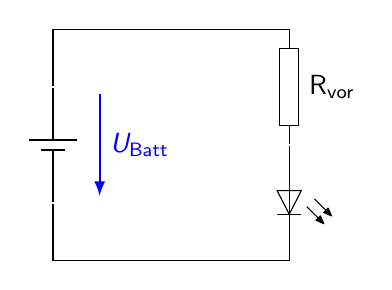
\begin{tikzpicture}[%show background rectangle,
circuit ee IEC, circuit symbol lines/.style={draw,thick},
font=\sffamily\upshape,
>=latex % Voreinstellung für Pfeilspitzen
]
\matrix (S) [
  matrix of nodes, nodes in empty cells,
  inner sep=0pt, outer sep=-.5\pgflinewidth,
  column sep=15mm, row sep = 7mm,
  nodes={minimum width=0pt}
  ]
{
  &&  \\
  &&  \\
  &&  \\
  &&  \\
  &&  \\
};
 
 
%Orientierungshilfen
%\foreach \j in {1,...,5}
% \foreach \k in {1,...,3}{%
%\node[text=lightgray] at (S-\j-\k){+}; % Orientierungshilfe +
%\node[red, left] at (S-\j-1){\j}; %Orientierungshilfe Zeilennummer
%\node[red, above] at (S-1-\k){\k}; %Orientierungshilfe Spaltennummer  
%};%
 

%Bauteile
\draw (S-2-1) to  [battery={name=Bat}](S-4-1);
\draw (S-1-3) to  [resistor={info=R$_\mathsf{vor}$, name=Wstd}](S-3-3);
\draw (S-3-3) to  [diode={light emitting}](S-5-3);


%Spannungspfeile
%Spannungspfeil der Quelle / des Voltmeters
\draw[UPfeil=0.25em] ([xshift=6mm]S-2-1.east) --
([xshift=6mm]S-4-1.east) node[midway, right]{U$\mathsf{_{Batt}}$};
 
%Leiterbahnen
\draw (S-1-1) -- (S-2-1);
\draw (S-1-1) -- (S-1-3);
\draw (S-4-1) -- (S-5-1);
\draw (S-5-1) -- (S-5-3); 

\end{tikzpicture}
\end{center}
Widerstand der LED im Betrieb
\[R_{LED}=\frac{U_{LED}}{I_{LED}}=\frac{2V}{20mA}=100\Omega\]
Ein Vorwiderstand wird mit der LED in Reihe geschalten, also addieren sich Der Vorwiderstand und der Widerstand der LED zum Gesamtwiderstand der Schaltung. 
\begin{align}
 R_{G} & = R_{vor}+R_{LED} \nonumber \\ 
 \frac{U_{Batt}}{I_{LED}} & = R_{vor} + \frac{U_{LED}}{I_{LED}} \nonumber \\
 R_{vor} & = \frac{U_{Batt}}{I_{LED}}-\frac{U_{LED}}{I_{LED}} \nonumber \\
 		 & = \frac{U_{Batt} - U_{LED}}{I_{LED}} \nonumber \\
 		 & = \frac{12V - 2V}{20mA} \nonumber \\
 R_{vor} & = 500\Omega \nonumber 
\end{align}
Es wird also ein Vorwiderstand mit $ R_{vor} = 500\Omega $ in der Schaltung benötigt.


%%%
%%% end main document
%%%
%%%%%%%%%%%%%%%%%%%%%%%%%%%%%%%%%%%%%%%%%%%%%%%%%%%%%%%%%%%%%%%%%%%%%%%%%%%%%%%%

% \appendix  %% include it, if something (bibliography, index, ...) follows below

%%%%%%%%%%%%%%%%%%%%%%%%%%%%%%%%%%%%%%%%%%%%%%%%%%%%%%%%%%%%%%%%%%%%%%%%%%%%%%%%
%%%
%%% bibliography
%%%
%%% available styles: abbrv, acm, alpha, apalike, ieeetr, plain, siam, unsrt
%%%
% \bibliographystyle{plain}

%%% name of the bibliography file without .bib
%%% e.g.: literatur.bib -> \bibliography{literatur}
% \bibliography{FIXXME}

\end{document}
%%% }}}
%%% END OF FILE
%%%%%%%%%%%%%%%%%%%%%%%%%%%%%%%%%%%%%%%%%%%%%%%%%%%%%%%%%%%%%%%%%%%%%%%%%%%%%%%%
%%% Notice!
%%% This file uses the outline-mode of emacs and the foldmethod of Vim.
%%% Press 'zi' to unfold the file in Vim.
%%% See ':help folding' for more information.
%%%%%%%%%%%%%%%%%%%%%%%%%%%%%%%%%%%%%%%%%%%%%%%%%%%%%%%%%%%%%%%%%%%%%%%%%%%%%%%%
%% Local Variables:
%% mode: outline-minor
%% OPToutline-regexp: "%% .*"
%% OPTeval: (hide-body)
%% emerge-set-combine-versions-template: "%a\n%b\n"
%% End:
%% vim:foldmethod=marker
